\documentclass{tufte-handout}
\usepackage{graphicx}
\graphicspath{ {./images/} }

\title{Kernel Methods}
\author{Andr\'es Ponce}
\begin{document}
\maketitle
\begin{abstract}

\textbf{Kernel methods} allow us to find
patterns in data, useful for classification
and regression. These methods allow us to quickly
and efficiently work with high dimensional data.
We break down a function that might not be linear
in nature to linear functions of its components. 
$k(x,y) = (f(x), g(y))$, where $f$ and $g$ are the 
dimensional inputs.
\end{abstract}

\section{Dual representations}
	\subsection{Parametric vs. non-parametric models}
	\textbf{Parametric methods} refer to when we train a model that
	is a function of $y(x, w)$, where we map x to y. In this scenario,
	the training data are thrown away after training.

	On the other hand, \textbf{non-parametric methods} use a nearest-neighbor
	classifier strategy to perform classification. However, in this scheme we 
	keep the training data.
	
	Kernel methods evaluate a \textbf{kernel function} based on the training
	data. The dual part of this representation comes from the kernel function
	itself. We define a basic kernel function as: \footnote{Notice this function 
	is \textbf{symmetric}, since $k(x, x') = k(x', x)$}
	\[k(x, x') = \phi(x)^{T}\phi(x')\]

	Based on this formulation, we can then define vector $a$, which we use instead
	of the weight vector $w$. What $a$ allows us to rephrase the optimal solution
	as a linear combination of the entire training data set. We define $a$:
	\footnote{$a$ is the result of setting the derivative of $J(w)$ to zero, where $J(w)$
	is a sum of squares formultion}
	\[a_{n} = -\frac{1}{\lambda}\{w^{T}\phi(x_{n}) - t_{n}\}\]

	Then, we next define the \textbf{Kernel Matrix} $K = \Phi\Phi^{T}$, which makes $K$ a
	symmetric matrix with each cell in the matrix:
	\[ K_{nm} = \phi(x_{n})^{T}\phi(x_{m}) = k(x_{n}, x_{m})\]
	Finally, the solution again is of the form $y(x) = w^{T}\phi(x)$, however with the 
	new concepts we've introduced we can write the final solution as
	\[k(x)^{T}(K + \lambda I_{N})^{-1}t\]

	\subsection{Final notes on Dual representations}
	If we have $M$ dimensions in our data, with $N$ data points, we will usually have 
	more data points than dimensions in our data. This might make dual representations
	less efficient and might lead to more sparse matrices in the end. However, since
	we don't take into account the feature set of our data $\phi(x)$, we can handle 
	data with potentially infinite features, making it more flexible.
\section{Constructing Kernels}
	How do we build a kernel to lead to more accurate classification? Maybe we can first find
	a feature space for its inputs and then check if there is a space where the output is equal to 
	the inner product of the data points (i.e. $y(x) = k(f(x), g(x')$). 
	So when we multiply the inner products in some lower dimensional space, the result exists in a 
	higher space where we are wanting to find the kernel anyways.\footnote{Maybe this is why it's used
	in facial recognition? Becuase each pixel in an image can correpsond to a dimension in the data,
	we want to break it down to a combination of lower dimensions.}

	Once we find a candidate function, how canwe show it's a proper kernel function? We can know its 
	a valid kernel function by calculating its eigenvalues. If all its eigenvalues are positive,
	then the matrix $K$ is \textbf{positive} and \textbf{semi-definite}.
	
	Some types of kernel functions: 
	\begin{itemize}
		\item \textbf{Polynomial kernel}: $k(x, x') = (x^{T}x' + c)^{M}$
				
				Similar to our basic kernel function,this one is symmetric.
		\item \textbf{Gaussian kernel}: $k(x, x') = \textrm{exp}(-\|x - x'\|^{2})$
		\item \textbf{Sigmoidal kernel}: $k(x, x') = \textrm{tanh}(\alpha x^{T}x' + b)$
				where a and b are constants. The Gram matrix of this function is usually not
				positive or semi-definite, however it can be useful in practice.
	\end{itemize}

\section{Support Vector Machines for classification}
	\subsection{Maximum Margin classifier}
		Suppose we have $N$ training data points and their corresponding labels $t$. SVMs use
		a normal-enough looking formula like 
		\[y(x) = w^{T}\phi(x) + b\]
		where $\phi(x)$ denotes the fixed feature-space transformation.
		
		If we have linearly separable classes, we can have multiple decision boundaries that
		give adequate solutions. Is there an optimal one, though? If so, how do we calculate that?

		\begin{marginfigure}		
			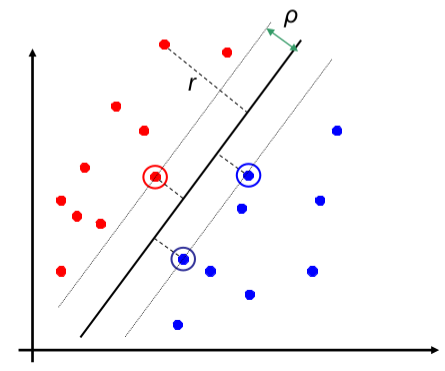
\includegraphics[scale=0.3]{margin}
			\caption{The margin is the smallest distance between the decision boundary and any of
				the training points.}
		\end{marginfigure}	

		We want to maximize the \textbf{margin}, since a greater distance would mean that the data is 
		split more cleanly along the decision boundary. Then the perpendicular distance between the 
		decision boundary and the data point is given by 
		\[ \frac{t_{n}y(x_{n})}{\|w\|} = \frac{t_{n}(w^{T}\phi(x_{n}) + b)}{\|w\|}\]
		which is the equation we want to maximize.
		
		Here we can also use Lagrangian multipliers to find an optimization. The optimization can be done
		in $O(n^{3})$.
		
		According to the \textbf{KKT} conditions, we can have three conditions regarding SVMs:
		\begin{enumerate}
			\item $a_{n} \geq 0$
			\item $t_{n}y(x_{n}) -1 \geq 0$
			\item $a_{n}\{t_{n}y(x_{n})-1\} = 0$
		\end{enumerate}
		Due to the third contstraint above, either $a_{n} = 0$ or $t_{n}y(x_{n}) - 1 = 0$. If the former
		is true, then the point is of no importance when applying the decision function.

		If the latter is true and $t_{n}(x_{n}) - 1 -0$, then this point lies on the maximum margin and 
		is called a \textbf{support vector}. We only keep the support vectors.
\end{document}
